\documentclass[a4paper, 14pt]{extarticle}
\renewcommand{\baselinestretch}{1.5}

\usepackage{indentfirst}
\usepackage{geometry}
\usepackage{float}
\usepackage[nottoc]{tocbibind}
\usepackage{amsmath} % Advanced math typesetting
\usepackage[utf8]{inputenc} % Unicode support (Umlauts etc.)
\usepackage[T2A]{fontenc} % Unicode support (Umlauts etc.)
\usepackage[russian]{babel} % Change hyphenation rules
\usepackage{hyperref} % Add a link to your document
\usepackage{graphicx} % Add pictures to your document
\usepackage{caption}
\numberwithin{figure}{subsection}
\let\oldautoref\autoref
\renewcommand{\autoref}[1]{(\oldautoref{#1})}

\usepackage{listings} % Source code formatting and highlighting

\usepackage{titlesec}
\titleformat{\section}{\normalfont\large\bfseries}{Глава \thesection}{1em}{}

\usepackage[titles]{tocloft}
\renewcommand{\cftsecpresnum}{Глава\space}
\newlength\mylength
\settowidth\mylength{\cftsecpresnum}
\addtolength\cftsecnumwidth{\mylength}

\numberwithin{equation}{subsection}

\usepackage{amsthm}
\newtheorem{theorem}{Теорема}[subsection]
\newtheorem{definition}{Определение}[subsection]
\newtheorem{example}{Пример}[subsection]
\newtheorem{algorithm}{Алгоритм}[subsection]

\usepackage[shortlabels]{enumitem}

\begin{document}
\bibliographystyle{utf8gost705u}
\thispagestyle{empty}
\begin{center}
\small{Федеральное государственное автономное образовательное учреждение высшего профессионального образования \\ «Московский физико-технический институт (государственный университет)»

Факультет Аэрофизики и Космических Исследований

Кафедра Логистические Системы и Технологии}

\parskip=80pt
КУЗЬМИНА Антонина Ильинична
\parskip=30pt

\textbf{\large{Математическое моделирование конвейера принятия торговых решений трейдером фондовой биржи}}

ДИПЛОМНАЯ РАБОТА
\end{center}

\begin{flushright}
\parskip=50pt
Научный руководитель:
\end{flushright}

\vspace{\fill}
\begin{center}
Москва, 2016
\end{center}
\newpage{}
\tableofcontents{}
\newpage{}
\addcontentsline{toc}{section}{Введение}
\section*{Введение}
В последнее время большое количество людей занимается торговлей на бирже — по
некоторым оценкам, около 800 тысяч человек. О популярности этой сферы деятельности
свидетельствует также и объем торгов на московской бирже, растущий день ото дня и
составивший 4.65 трлн рублей 16 декабря 2014 года.

В то же время, игра на бирже является очень рискованным видом деятельности — до 80\%
участников торгов терпят убытки. Поэтому трейдер никогда не принимает решений по
наитию, а всегда использует холодный расчет. Вследствие этого, как правило, большинство
торговых стратегий довольно легко формализуемы.

Автоматические торговые системы имеют большое количество преимуществ по сравнению с
трейдером-человеком. Самые значительные из них заключаются в следующем:

\begin{itemize}
\item Торговый робот может торговать круглосуточно, не отвлекаясь на еду и сон.
\item Торговый робот не отнимает ценное время человека --- можно запустить
одновременно несколько роботов и, в то же время, заниматься созданием новых
стратегий.
\item Торговый робот принимает все решения в строгом соответствии с логикой алгоритма,
он готов терпеть просадки и не берет на себя лишний риск, что очень важно в
условиях высоковолатильного рынка.
\item Торговый робот способен принимать решения гораздо быстрее любого человека ---
если трейдеру для совершения сделки требуется не менее 0.5 секунды, робот способен
совершить сделку уже через 2-3 мкс.
\end{itemize}

Объектом исследования в данной работе является конвейер принятия решений трейдером фондовой биржи.

Основной целью данной работы является разработка математической модели конвейера принятия решений трейдером фондовой биржи, а также ее практическая реализация и проверка на реальных данных как всей моделирующей программы в целом, так и ее отдельных частей.

Для достижения цели настоящей работы поставлены следующие задачи:

\begin{itemize}
\item Исследование существующих методов моделирования работы трейдера.
\item Исследование существующих открытых источников финансовой информации
(котировок различных активов, а также торговых индикаторов) и принятие решения.
об использовании этих данных для построения и тестирования модели конвейера принятия торговых решений трейдером фондовой биржи
\item Исследование существующих открытых источников информации о фигурах технического анализа для использования этих данных при построении модели.
\item Изучение существующей научной литературы по вопросу поиска известных паттернов в истории котировок финансовых инструментов.
\item Выбор метрик расстояния между свечами для использования при реализации алгоритма динамического искажения времени.
\item Реализация алгоритма динамического искажения времени для поиска известного паттерна в истории котировок торгового инструмента в среде программирования Microsoft Visual Studio с использованием языка программирования C\#.
\item Тестирование программы поиска известного паттерна в истории котировок торгового инструмента на реальных исторических данных с использованием методов модульного и функционального тестирования.
\item Определение качества работы программы поиска известного паттерна на реальных исторических данных посредством проведения слепого исследования, а также сравнение достигнутого уровня качества работы при использовании различных метрик расстояния.
\item Изучение существующих методов кластерного анализа.
\item Реализация различных методов кластеризации для поиска новых паттернов в истории котировок финансовых инструментов в среде программирования Microsoft Visual Studio с использованием языка программирования C\#.
\item Тестирование программы поиска новых паттернов в истории котировок торгового инструмента с применением алгоритмов кластеризации на реальных исторических данных с использованием методов модульного и функционального тестирования.
\item Определение качества работы программы поиска новых паттернов в истории котировок торгового инструмента с применением алгоритмов кластеризации на реальных исторических данных посредством проведения слепого исследования, а также сравнение качества работы различных методов кластеризации между собой.
\item Реализация торговой системы, основанной на использовании найденных фигур технического анализа, в среде программирования Microsoft Visual Studio с использованием языка программирования C\#.
\item Тестирование торговой системы, основанной на использовании найденных фигур технического анализа, на реальных исторических данных и определение важнейших параметров этой торговой системы (прибыль, просадка и тд.).
\item Реализация алгоритма-советника для торговой платформы MetaTrader для проверки
торговой системы на демо-счете в режиме реального времени.
\end{itemize}

Теоретической основой исследования явились положения и концепции, представленные в
работах отечественных и зарубежных авторов по проблемам:

\begin{itemize}
\item Численной оптимизации.
\item Поиска паттернов во временных рядах.
\item Алгоритма динамического искажения времени.
\item Классической и вероятностной постановки задач машинного обучения.
\item Эвристических, статистических и иерархических методов кластеризации, в том числе, с использованием нейронных сетей.
\item Переобучения и мультиколлинеарности, а также методам борьбы с этими проблемами:
регуляризации, выделению главных компонент и др.
\item Сравнения качества работы различных алгоритмов машинного обучения.
\item Технического анализа.
\end{itemize}

Вопросы, рассматриваемые в данной работе, нашли отражение в трудах таких классических авторов, как Колмогоров, Вапник, Червоненкис, Закс и Стоун.

Среди современных ученых схожими проблемами занимаются Воронцов, Горбань, Халл, Алексис, Бушерон, Тибширани, Руммельхарт, Носедал, Райт, Куликов.

Работа состоит из введения, трех глав, заключения и списка литературы.

В первой главе приведены экономические термины, необходимые для понимания работы, описаны этапы конвейера принятия решений трейдером фондовой биржи, а также приведена формальная постановка задач, рассматривающихся в работе.

Вторая глава представляет собой теоретическое введение к описанию экспериментов, проведенных в рамках данной работы. В нем описаны алгоритмы, примененные при написании программы: алгоритм динамического искажения времени (а также его модификация, алгоритм derivative dynamic time warping, и используемые метрики расстояния в пространстве историй котировок) и алгоритмы кластеризации (эвристические, статистические и иерархические методы кластеризации, а также самоорганизующиеся карты Кохонена). Приведены основные теоремы, связанные с гарантиями сходимости используемых методов.

В третьей главе описываются результаты, полученные в ходе практической реализации алгоритмов и тестирования их на реальных исторических данных.
\section{Постановка задач}
\subsection{Необходимые термины}
Ниже приведены определения финансовых терминов, использующиеся в работе.

{\it Актив} --- некоторая сущность, которая может быть куплена или продана в любой момент времени по цене, соответствующей этому моменту времени. Цены покупки и продажи актива в один и тот же момент времени не обязаны совпадать.

{\it Тик} --- сделка купли-продажи, произошедшая на бирже. Характеризуется моментом времени, ценой и объемом. Объем сделки --- количество элементарных единиц актива, которые были проданы продавцом и куплены покупателем.

{\it Свеча} --- элемент данных, представляющий собой консолидированную информацию об изменении цены актива в некоторый промежуток времени. Как правило, свеча включает в себя 4 величины: цену открытия интервала (цена первого тика из временного интервала), цену закрытия (цена последнего тика из временного интервала), а также максимальную и минимальную цены тиков из рассматриваемого временного интервала. Нередко также в состав свечи включают общий объем всех сделок, произошедших в течение рассматриваемого промежутка времени, однако в данной работе эта величина не используется.

{\it Торговая система} --- алгоритм, совершающий сделки на бирже по определенным математическим правилам. Может иметь параметры, влияющие на поведение системы.

{\it Сделка покупки актива} --- сделка по покупке-продаже актива, в которой рассматриваемая торговая система выступает в качестве покупателя.

{\it Сделка продажи актива} --- сделка по покупке-продаже актива, в которой рассматриваемая торговая система выступает в качестве продавца.

{\it Закрытая сделка} --- пара сделок с совпадающими объемами, состоящая из сделки по покупке актива и сделки по продаже актива.

{\it Ряд данных} --- последовательность данных о цене актива за определенный промежуток времени. Как правило, включает в себя информацию обо всех свечах этого актива за данный промежуток времени.

{\it Прибыль закрытой сделки} --- разность цен сделок продажи и покупки этой закрытой сделки, умноженная на объем этих сделок.

{\it Прибыль торговой системы за некоторый интервал времени.} Обозначим $n$ общее число закрытых сделок торговой системы за рассматриваемый период. Обозначим $p_i,~i=1,...,n$ прибыль $i-$ой закрытой сделки. Тогда прибылью торговой системы называется величина $profit=\sum\limits_{i=1}^n{p_i}$.

{\it Просадка торговой системы за некоторый интервал времени.} Обозначим $n$ общее число закрытых сделок торговой системы за рассматриваемый период. Обозначим $p_i,~i=1,...,n$ прибыль $i-$ой закрытой сделки. Тогда просадкой торговой системы называется величина $$drawdown=\max\limits_{i=1,...,n}\left(\max\limits_{k=1,...,i}\sum\limits_{j=1}^kp_j - \sum\limits_{j=1}^ip_j\right)$$

{\it Функционал качества торговой системы} --- некоторая функция, характеризующая качество торговой системы. Как правило, для ее вычисления используется последовательность закрытых сделок торговой системы. Типичные примеры функционала качества --- $profit$ и $profit/drawdown$.
\subsection{Этапы конвейера принятия решений трейдером фондовой биржи}
В данной работе рассматривается трейдер фондовой биржи, принимающий торговые решения на основе фигур технического анализа. Конвейер принятия решений в этом случае включает в себя следующие этапы:

\begin{enumerate}
\item Поиск закономерностей фондового рынка
\begin{enumerate}
\item Выделение типичных фигур технического анализа
\item Определение информативности каждой фигуры технического анализа
\end{enumerate}
\item Создание торговой стратегии
\begin{enumerate}
\item Поиск фигур технического анализа в биржевых данных в режиме реального времени
\item Принятие торгового решения и совершение сделки
\item Оптимизация торговой стратегии
\item Запуск автоматической торговой системы
\end{enumerate}
\end{enumerate}

В данной работе рассматриваются все этапы этого конвейера, однако основное внимание уделяется трем задачам: задаче поиска известного паттерна в истории котировок, задаче кластеризации в пространстве фрагментов историй котировок и задаче автоматизированного построения эффективной торговой стратегии.

\subsection{Постановка задач}
\subsubsection{Задача поиска известного паттерна в истории котировок}

Введем следующие обозначения:

$X^l = \{x_i\}_{i=1}^l$ - набор данных об истории котировок торгового инструмента, то есть,
\begin{itemize}
\item $x_i.open$ --- цена открытия $i$-ой свечи;
\item $x_i.high$ --- цена максимума $i$-ой свечи;
\item $x_i.low$ --- цена минимума $i$-ой свечи;
\item $x_i.close$ --- цена закрытия $i$-ой свечи.
\end{itemize}

$P^n = \{p_i\}_{i=1}^n$ --- паттерн для поиска в истории котировок, в виде последовательности свечей.

$Y \in \{0, 1\}^{l \times l}$ --- набор известных ответов (ground truth). $y_{ij} = 1$ обозначает, что подстрока котировок с $i$-ой по $j$-ую свечу включительно является вхождением искомого паттерна, а $y_{ij} = 0$ - что не является.

$a: \{1, \dots, l\} \times \{1, \dots, l\} \rightarrow \{0, 1\}$ --- построенный алгоритм. $a(i, j) = 1$ обозначает, что подстрока котировок с $i$-ой по $j$-ую свечу включительно является вхождением искомого паттерна, а $a(i, j) = 0$ - что не является.

$L(a, y) = 
\begin{cases}
0, a = y;\\
1, a \ne y
\end{cases}$ --- функция потерь, хакактеризующая величину ошибки алгоритма, выдавшего ответ $a$, на объекте с верным ответом $y$.

$Q(a, X^l, Y^{l \times l}) = {1 \over {l^2}}\sum_{i=1}^l\sum_{j=1}^l L(a(i, j), y_{ij})$ --- функционал качества алгоритма $a$.

Задачу поиска паттерна в истории котировок можно сформулировать следующим образом:

\begin{equation}
	\mu(X^l, Y^{l \times l}) = \operatornamewithlimits{argmin}\limits_{a \in A} Q(a, X^l, Y^{l \times l}).
\end{equation}

\subsubsection{Задача кластеризации в пространстве фрагментов историй торгов}
\subsubsection{Задача построения эффективной торговой стратегии}
\section{Теоретическое введение}
\subsection{Алгоритм динамического искажения времени}
Динамическое искажение времени (DTW) является широко известной техникой поиска оптимального соответствия между двумя временными последовательностями \autoref{fig:p1}. Грубо говоря, последовательности искажаются нелинейным образом для достижения максимального соответствия. Впервые DTW был применен для сравнения различных паттернов при распознавании голоса \cite{wjb87}.  В таких областях, как анализ данных и получение информации, DTW был успешно применен для автоматического распознавания искажений времени и различий в скоростях временных рядов.

В этой главе вводятся и обсуждаются основные идеи классического алгоритма DTW, а также приводятся его различные модификации, касающиеся как локального, так и глобального поведения алгоритма.

\begin{figure}[h]
\centering
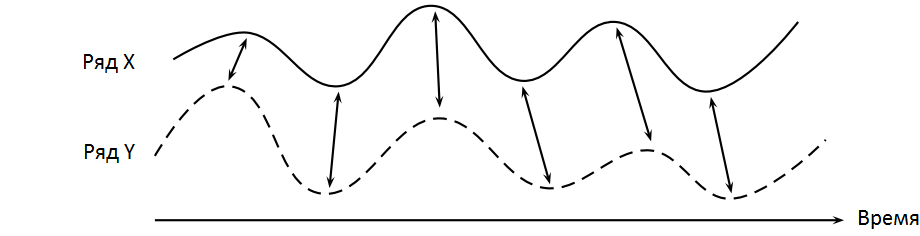
\includegraphics[width=15cm]{p1.png}
\caption{Сопоставление двух временных рядов. Соответствующие пары точек указаны стрелками.}
\label{fig:p1}
\end{figure}

\subsubsection{Базовый алгоритм динамического искажения времени}
Целью DTW является сравнение двух последовательностей данных $X = (x_i)_{i=1}^n$ длины $n$ и $Y = (y_i)_{i=1}^m$ длины $m$. Эти последовательности данных могут быть как дискретными сигналами (временными рядами), так и, в более общем случае, последовательностями любых объектов, расположенных через одинаковые промежутки времени друг от друга. Обозначим пространство признаков $F$. Тогда $x_i \in F$, для $i \in [1, \dots, n]$, и $x_i \in F$, для $i \in [1, \dots, m]$. Для сравнения двух различных элементов $x, y \in F$, требуется наличие локальной меры стоимости, также называемой локальной мерой расстояния, определяющейся функцией
\begin{equation}
	c: F \times F \rightarrow {\rm I\!R}_{\ge 0}.
\end{equation}
Обычно, $c$ такова, что ее значения невелики, если $x$ и $y$ близки друг к другу (или в некотором смысле похожи), и велики в противном случае. Посредством вычисления метрики расстояния для каждой пары элементов двух данных последовательностей получается матрица стоимости \autoref{fig:p2}, определенная следующим образом:
\begin{equation}
	C \in {\rm I\!R}^{n \times m},\> c_{ij} = c(x_i, y_j).
\end{equation}

\begin{figure}[h]
\centering
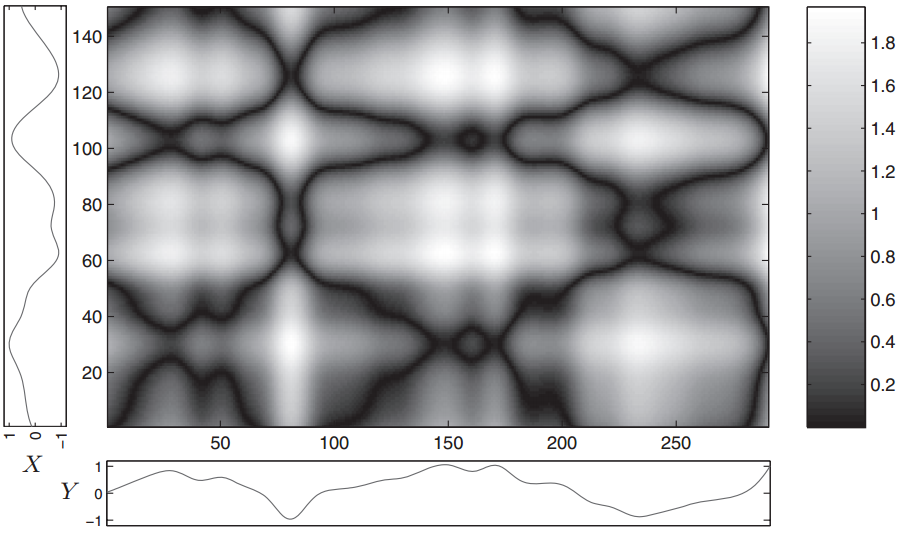
\includegraphics[width=15cm]{p2.png}
\caption{Матрица стоимости для двух вещественнозначных последовательностей X (вертикальная ось) и Y (горизонтальная ось) с использованием манхеттенского расстояния в качестве локальной меры расстояния. Регионы с меньшей стоимостью показаны черным цветом, с наибольшей - белым.}
\label{fig:p2}
\end{figure}
Таким образом, цель работы алгоритма DTW заключается в нахождении соответствия между последовательностями $X$ и $Y$, имеющего минимальную суммарную стоимость. Интуитивно, такое оптимальное соответствие должно проходить вдоль "долин" низкой стоимости в матрице стоимости \autoref{fig:p3}. Следующие определения формализуют понятие соответствия.

\begin{definition} \label{def:1}
	$(n, m)$-искажающий путь (также называемый просто искажающим путем, если $n$ и $m$ очевидны из контекста) --- это последовательность $p=(p_1, \dots, p_l),$ где $p_k = (i_k, j_k) \in [1, \dots, n] \times [1, \dots, m]$ для $i \in [1, \dots, l],$ удовлетворяющая следующим трем условиям.
\begin{enumerate}
\item Граничное условие: $p_1 = (1, 1)$ и $p_l = (n, m).$
\item Условие монотонности: $i_1 \le i_2 \le \dots \le i_l, j_1 \le j_2 \le \dots \le j_l$.
\item Условие размера шага: $p_{k+1}-p_{k} \in \{(0,1),(1,0),(1,1)\}$ для $k \in [1, \dots, l - 1].$
\end{enumerate}
\end{definition}

Условие монотонности является прямым следствием условия размера шага, однако, все же упомянуто для наглядности. $(n, m)$-искажающий путь $p=(p_1, \dots, p_l)$ определяет соответствие между двумя последовательностями $X=(x_1, \dots, x_n)$ и $Y=(y_1, \dots, y_m)$. Элементу $x_{i_k}$ здесь соответствует элемент $y_{j_k}$. Смысл граничного условия заключается в требовании соответствия между первыми и последними элементами последовательностей, другими словами, соответствие устанавливается между целыми последовательностями $X$ и $Y$, а не между некоторыми их составными частями. Условие монотонности отражает требование реалистичности времени: если некоторый элемент $x_i$ идет перед элементом $x_j$, то же самое должно выполняться для соответствующих им элементов последовательности $Y$, и наоборот. Наконец, условие размера шага является, в некотором роде, требованием непрерывности: каждый элемент каждой из последовательностей должен входить хотя бы в одну пару оптимального пути, и, в то же время, путь не должен иметь повторений в смысле одновременного равенства обеих компонент. Рисунок \ref{fig:p4} иллюстрирует эти три условия.

\begin{definition}
	Полной стоимостью искажающего пути $p=(p_1, \dots, p_l)$ между последовательностями $X = (x_1, \dots, x_n)$ и $Y = (y_1, \dots, y_m)$ относительно меры стоимости $c$ называется величина
\begin{equation}
	c_p(X, Y) = \sum_{k=1}^l c(x_{i_k}, y_{j_k});
\end{equation}
\end{definition}

\begin{definition}
	Оптимальным искажающим путем $p^*(X, Y)$ называется искажающий путь, имеющий наименьшую полную стоимость.
\end{definition}

\begin{definition}
	Расстоянием динамического искажения времени между последовательностями $X = (x_1, \dots, x_n)$ и $Y = (y_1, \dots, y_m)$ относительно меры стоимости $c$ называется величина
\begin{multline}
	DTW(X, Y, c) = c_{p^*}(X, Y) = \\ \min \{c_p(X, Y) | p - (n, m)-\text{искажающий путь}\}.
\end{multline}
\end{definition}

\begin{figure}[h]
\centering
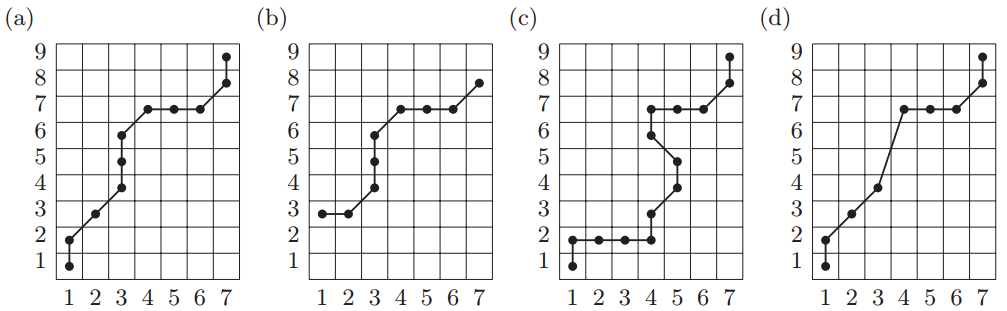
\includegraphics[width=15cm]{p4.png}
\caption{Иллюстрация некоторых вариантов искажающего пути для двух последовательностей: $X$ из 9 элементов и $Y$ из 7 элементов. {\bf (a)} Допустимый искажающий путь, удовлетворяющий условиям 1 - 3. {\bf (b)} Граничное условие нарушено. {\bf (c)} Условие монотонности нарушено. {\bf (d)} Условие размера шага нарушено.}
\label{fig:p4}
\end{figure}

Заметим, что расстояние DTW является корректно определенным даже в случае наличия нескольких искажающих путей минимальной полной стоимости. Кроме того, легко доказать, что расстояние DTW является симметричным, если локальная мера $c$ является симметричной. Однако, расстояние DTW может не являться положительно определенным даже в случае, если для исходной меры это так. Более того, расстояние DTW может не удовлетворять неравенству треугольника даже в случае, если $c$ является метрикой. Этот факт иллюстрируется следующим примером.

\begin{example}
	Пусть $F=(\alpha, \beta, \gamma)$ --- пространство признаков из трех элементов, $c(x, y) = 0$, если $x = y$ и $c(x, y) = 1$, если $x \ne y$ --- локальная мера расстояния. Очевидно, $c$ является метрикой над $F$ и удовлетворяет неравенству треугольника. Теперь рассмотрим $X=(\alpha,\beta,\gamma)$, $Y=(\alpha,\beta,\beta,\gamma)$ и $Z=(\alpha,\gamma,\gamma).$ Тогда $DTW(X,Y,c) = 0,$ $DTW(X, Z, c) = 1$, но $DTW(Y,Z, c) = 2.$
\end{example}

Оптимальный искажающий путь $p^*$ может быть найден перебором всех возможных искажающих путей, однако такой метод имеет экспоненциальную сложность. Далее в этом разделе будет приведен алгоритм, основанный на методе динамического программирования, и имеющий сложность $O(nm)$.

Обозначим $X(1:k)=(x_1, \dots, x_k)$ для $k \in [1, \dots, n]$ и $Y(1:k)=(y_1, \dots, y_k)$ для $k \in [1, \dots, m]$ префиксы последовательностей $X$ и $Y$.

\begin{definition}
	Аккумулированной матрицей стоимости называется матрица, определенная следующим образом:
\begin{equation}
	D \in {\rm I\!R}^{n \times m},\> d_{ij} = DTW(X(1:i), Y(1:j)).
\end{equation}
\end{definition}

Очевидно, $d_{nm} = DTW(X, Y)$. Следующая теорема показывает, что матрица $D$ может быть эффективно вычислена.

\begin{theorem} \label{thm:1}
	Матрица аккумулированной стоимости удовлетворяет следующим равенствам:
\begin{equation} d_{i1} = \sum_{k=1}^i c(x_k, y_1)\> \text{для}\> i \in [1, \dots, n]; \label{eq:1}\end{equation}
\begin{equation} d_{1i} = \sum_{k=1}^i c(x_1, y_k)\> \text{для}\> i \in [1, \dots, m];\label{eq:2} \end{equation}
\begin{multline}
d_{ij} = \min\{d_{i-1 j-1},d_{i j-1},d_{i-1 j}\} + c(x_i, y_j)\\ \text{для}\> i \in [1, \dots, n]\> \text{и}\> j \in [1, \dots, m]. \label{eq:3}
\end{multline}
В частности, $DTW(n,m)$ может быть вычислено за $O(nm)$ операций.
\end{theorem}
{\it Доказательство.}
\begin{enumerate}
\item Пусть $i=1$ и $j \in [1, \dots, m]$. Тогда существует единственный искажающий путь для $X(1:i)$ и $Y(1:j)$, имеющий полную стоимость $\sum_{k=1}^j c(x_1, y_k)$. Формула (\ref{eq:1}) доказана.
\item Аналогично доказывается формула (\ref{eq:2}).
\item Положим $i > 1$ и $j > 1$. Пусть $q = (q_1, \dots, q_l)$ --- оптимальный искажающий путь для префиксов $X(1:i)$ и $Y(1:j).$
\item Тогда, в соответствии с граничным условием, $q_l = (i, j).$
\item Обозначим $(a, b) = q_{l-1}.$ В соответствии с условием размера шага, $(a, b) \in \{(i-1, j-1),(i,j-1),(i-1,j)\}$.
\item Кроме того, $(q_1, \dots, q_{l-1})$ должна быть оптимальным искажающим путем для $X(1:a)$ и $Y(1:b)$.
\item Поскольку $d_{ij} = c_{q_1, \dots, q_{l-1}}(X(1:a), Y(1:b)) + c(x_i, y_j),$ из отпимальности искажающего пути $q$ следует истинность (\ref{eq:3}).
\end{enumerate}

Из теоремы \ref{thm:1} следует возможность построения алгоритма рекурсивного вычисления аккумулированной матрицы расстояний за вреия $O(nm)$. Инициализация, производящаяся в алгоритме, может быть упрощена, если положить $d_{0 i} = \infty$ для $i \in [1, \dots, m]$, $d_{i 0} = \infty$ для $i \in [1, \dots, n]$ и $d_{0 0} = 0.$

Более того, вычисления могут производиться построчно (или по столбцам), при этом, для вычисления очередной строки (столбца) матрицы $D$ требуется знание только одной предыдущей строки (столбца). Таким образом, вычисление $DTW(X, Y)$ требует $O(nm)$ времени и $O(\min(n,m))$ памяти. Кроме того, если требуется восстановление оптимального искажающего пути, эта оптимизация неприменима, и потребуется $O(nm)$ памяти.

Ниже приводятся два алгоритма: алгоритм вычисления матрицы кумулятивного расстояния и алгоритм восстановления оптимального искажающего пути по матрице кумулятивного расстояния.

\begin{algorithm} {\bf AccumulatedCostMatrix}

{\bf Исходные данные:} Последовательности $X$ и $Y$, а также мера локального расстояния $c$.

{\bf Результат работы:} Матрица кумулятивного расстояния $D$.
\begin{enumerate}[parsep = 0pt]
\item {\bf Инициализация:}
\begin{enumerate}[1.,labelindent=0pt,labelsep=40pt,parsep = 0pt]
\setcounter{enumii}{\number\numexpr\value{enumi}}
\item $d_{0 0} = 0;$
\item Для $i=1,\dots,n:$
\begin{enumerate}[1.,labelindent=0pt,labelsep=80pt,parsep = 0pt]
\setcounter{enumiii}{\number\numexpr\value{enumii}}
\item $d_{i 0} = \infty$
\setcounter{enumii}{\number\numexpr\value{enumiii}}
\end{enumerate}
\item Для $i=1,\dots,m:$
\begin{enumerate}[1.,labelindent=0pt,labelsep=80pt,parsep = 0pt]
\setcounter{enumiii}{\number\numexpr\value{enumii}}
\item $d_{0 i} = \infty$
\setcounter{enumii}{\number\numexpr\value{enumiii}}
\end{enumerate}
\setcounter{enumi}{\number\numexpr\value{enumii}}
\end{enumerate}
\item {\bf Ход алгоритма:}
\begin{enumerate}[1.,labelindent=0pt,labelsep=40pt,parsep = 0pt]
\setcounter{enumii}{\number\numexpr\value{enumi}}
\item Для $i = 1,\dots, n:$
\begin{enumerate}[1.,labelindent=0pt,labelsep=80pt,parsep = 0pt]
\setcounter{enumiii}{\number\numexpr\value{enumii}}
\item Для $j=1,\dots,m:$
\begin{enumerate}[1.,labelindent=0pt,labelsep=140pt,parsep = 0pt]
\setcounter{enumiv}{\number\numexpr\value{enumiii}}
\item $d_{ij} = \min\{d_{i-1 j-1}, d_{i j-1}, d_{i-1 j}\} + c(x_i, y_j).$
\setcounter{enumiii}{\number\numexpr\value{enumiv}}
\end{enumerate}
\setcounter{enumii}{\number\numexpr\value{enumiii}}
\end{enumerate}
\setcounter{enumi}{\number\numexpr\value{enumii}}
\end{enumerate}
\end{enumerate}
\end{algorithm}

На рисунке \ref{fig:p3} изображен оптимальный искажающий путь для последовательностей с рисунка \ref{fig:p2}.

\begin{figure}[H]
\centering
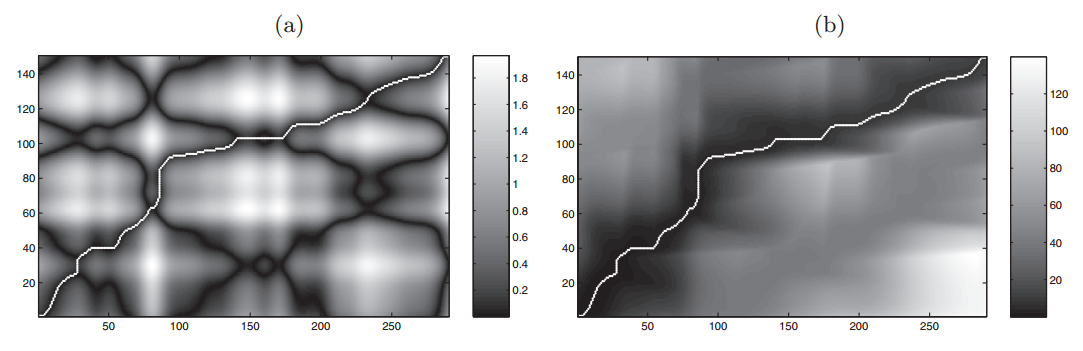
\includegraphics[width=15cm]{p3.png}
\caption{Матрица стоимости, взятая с \oldautoref{fig:p2}, и кумулятивная матрица расстояния с отмеченным на них оптимальным путем}
\label{fig:p3}
\end{figure}

\begin{algorithm} {\bf OptimalWarpingPath}

{\bf Исходные данные:} Матрица кумулятивного расстояния $D$.

{\bf Результат работы:} Оптимальный искажающий путь $p^*$.
\begin{enumerate}[parsep = 0pt]
\item {\bf Инициализация:}
\begin{enumerate}[1.,labelindent=0pt,labelsep=40pt,parsep = 0pt]
\setcounter{enumii}{\number\numexpr\value{enumi}}
\item $p = {(n, m)};$
\item $(a, b) = (n, m);$
\setcounter{enumi}{\number\numexpr\value{enumii}}
\end{enumerate}

\item {\bf Ход алгоритма:}
\begin{enumerate}[1.,labelindent=0pt,labelsep=40pt,parsep = 0pt]
\setcounter{enumii}{\number\numexpr\value{enumi}}
\item Пока $(a, b) \ne (1,1):$
\begin{enumerate}[1.,labelindent=0pt,labelsep=80pt,parsep = 0pt]
\setcounter{enumiii}{\number\numexpr\value{enumii}}
\item Если $a = 1:$
\begin{enumerate}[1.,labelindent=0pt,labelsep=147pt,parsep = 0pt]
\setcounter{enumiv}{\number\numexpr\value{enumiii}}
\item $(a,b)=(a,b-1);$
\setcounter{enumiii}{\number\numexpr\value{enumiv}}
\end{enumerate}
\item Иначе, если $b = 1:$
\begin{enumerate}[1.,labelindent=0pt,labelsep=147pt,parsep = 0pt]
\setcounter{enumiv}{\number\numexpr\value{enumiii}}
\item $(a,b)=(a-1,b);$
\setcounter{enumiii}{\number\numexpr\value{enumiv}}
\end{enumerate}
\item Иначе:
\begin{enumerate}[1.,labelindent=0pt,labelsep=147pt,parsep = 0pt]
\setcounter{enumiv}{\number\numexpr\value{enumiii}}
\item $(a,b)=\arg\min{d_{a-1 b-1},d_{a b-1}, d_{a-1 b}};$
\setcounter{enumiii}{\number\numexpr\value{enumiv}}
\end{enumerate}
\item $p = \{(a,b), p\};$
\setcounter{enumii}{\number\numexpr\value{enumiii}}
\end{enumerate}
\setcounter{enumi}{\number\numexpr\value{enumii}}
\end{enumerate}
\end{enumerate}
\end{algorithm}

Ниже будут рассмотрены различные модификации алгоритма Dynamic Time Warping.

\subsubsection{Изменение условия на размер шага}
Напомним, что условие размера шага из определения \ref{def:1} является, в некотором смысле, условием непрерывности построенного искажающего пути, именно оно дает гарантию того, что каждому элементу последовательности $X=\{x_1,\dots,x_n\}$ ставится в соответствие элемент последовательности $Y=\{y_1,\dots,y_m\}$, и наоборот. Однако, тот вид условия, который приведен в определении \ref{def:1}, имеет один существенный недостаток: одному и тому же элементу одной из последовательностей может быть поставлено в соответствие много элементов другой последовательности. Таким образом, на искажающем пути могут появиться вертикальные или горизонтальные участки, как изображено на рисунке \ref{fig:p5}a. Интуитивно, искажающий путь может "застрять" в некотором элементе, что приводит к значительному замедлению одной из последовательностей (и соответствующему ускорению второй).

\begin{figure}[h]
\centering
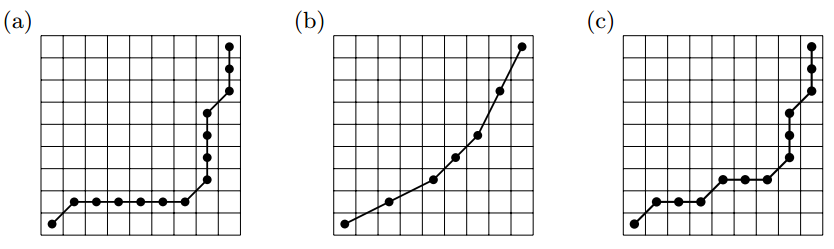
\includegraphics[width=15cm]{p5.png}
\caption{Искажающие пути, которые могут быть получены с применением условий размера шага, представленных на \oldautoref{fig:p6}: {\bf (a)} части искажающего пути вырождены, {\bf (b)} некоторым элементам последовательностей на соответствует ничего, {\bf (c)} Искажающий путь, лишенный этих недостатков.}
\label{fig:p5}
\end{figure}

\begin{figure}[H]
\centering
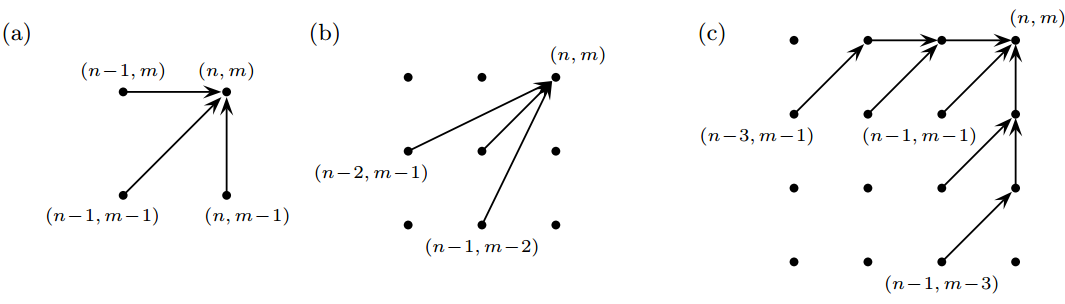
\includegraphics[width=15cm]{p6.png}
\caption{Иллюстрация различных условий размера шага. {\bf (a)} соответствует условию из определения \ref{def:1}.}
\label{fig:p6}
\end{figure}

Один из возможных способов избежать подобного вырождения заключается в изменении условия на размер шага для ограничения наклона рассматриваемых искажающих путей. Например, условие можно задать в виде

\begin{equation}
	p_i-p_{i-1} \in \{(2,1),(1,2),(1,1)\}\> \text{для} \> i \in [2,\dots,l].
\end{equation}

Такой вид ограничения размера шага приводит к наклону искажающего пути от $1 \over 2$ до $2$ (см. рис. \ref{fig:p5}b). В этом случае матрица кумулятивного расстояния может быть вычислена с использованием рекуррентного соотношения
\begin{equation}
	d_{ij}=\min\{d_{i-1 \> j-1}, d_{i-2 \> j-1}, d_{i-1 \> j-2}\} + c(x_i, y_j)
\end{equation}
для $i \in [2,\dots,n]$ и $j \in [2,\dots,m]$ и соответствующих начальных значений. При использовании такого ограничения на размер шага, искажающий путь между двумя последовательностями $X$ и $Y$ будет существовать только в случае, если их длины отличаются не более, чем вдвое. Кроме того, не для каждого элемента первой последовательности будет найден парный ему элемент второй последовательности (и наоборот). Эта ситуация показана на рисунке \ref{fig:p6}b.

Рисунок \ref{fig:p5}c иллюстрирует другой пример ограничения на размер шага, лишенного этих недостатков: это ограничение ограничивает наклон искажающего пути, но, в то же время, запрещает пропуск элементов последовательностей. Рекуррентное соотношение для матрицы кумулятивного расстояния в этом случае задается как

\begin{equation}
	d_{ij} = \min
\begin{cases}
	d_{i-1 \> j-1} + c(x_i, y_j),\\
	d_{i-2 \> j-1} + c(x_{i-1},y_j) + c(x_i,y_j),\\
	d_{i-1 \> j-2} + c(x_i,y_{j-1}) + c(x_i,y_j),\\
	d_{i-3 \> j-1} + c(x_{i-2},y_j) + c(x_{i-1},y_j) + c(x_i,y_j),\\
	d_{i-1 \> j-3} + c(x_i,y_{j-2}) + c(x_i,y_{j-1}) + c(x_i,y_j)
\end{cases}
\end{equation}
для $(i,j) \in [1,\dots,n] \times [1,\dots,m] \textbackslash \{(1,1)\}$. Здесь в качестве начальных значений можно использовать $d_{1 1} = c(x_1,y_1), d_{i \> -2} = d_{i \> -1} = d_{i \> 0} = \infty$ для $i \in [-2,\dots, n]$ и $d_{-2 \> i} = d_{-1 \> i} = d_{0 \> i} = \infty$  для $i \in [-2,\dots, m]$.

Такой вид ограничения на размер шага ограничивает наклон искажающего пути значениями $1 \over 3$ и $3$. Рисунок \ref{fig:p5} показывает отличия оптимального искажающего пути при использовании рассмотренных здесь условий размера шага.

\subsubsection{Добавление локальных весов}

Для того, чтобы поощрить использование алгоритмом горизонтальных, вертикальных или диагональных ходов, можно ввести вектор локальных весов $(w_d,w_h,w_v) \in {\rm I\!R}^3.$ В этом случае рекуррентные соотношения могут быть записаны в виде

\begin{equation}
d_{ij} = \min
\begin{cases}
d_{i-1 \> j-1} + w_d \cdot c(x_i, y_j), \\
d_{i-1 \> j} + w_h \cdot c(x_i, y_j), \\
d_{i \> j-1} + w_v \cdot c(x_i, y_j),
\end{cases}
\end{equation}
где $i \in [2,\dots,n]$ и $j \in [2,\dots,m].$ Кроме того, $d_{i \> 1} = \sum_{k=1}^i w_h \cdot c(x_k, y_1)$ для $i \in [2,\dots,n]$ и $d_{1 \> i} = \sum_{k=1}^i w_v \cdot c(x_1, y_k)$ для $i \in [2,\dots,m]$.

Случай $(w_d,w_h,w_v) = (1,1,1)$ соответствует классическому DTW. В этом случае алгоритм, вероятно, будет отдавать предпочтение диагональным ходам, поскольку один диагональный ход соответствует комбинации горизонтального и вертикального ходов. Аналогично могут быть введены веса при использовании других видов ограничения на размер шага.

\subsubsection{Добавление глобальных ограничений}

Другим широко известным вариантом алгоритма DTW является введение глобальных ограничений на допустимые искажающие пути. Такие ограничения не только ускоряют вычисление DTW, но также предотвращают построение странных искажающих путей.

Более формально, назовем $R \subseteq [1,\dots,n] \times [1,\dots,m]$ глобальным ограничивающим регионом. Тогда искажающий путь относительно $R$ --- это искажающий путь, полностью лежащий внутри региона $R$. Оптимальный искажающий путь относительно $R$, обозначающийся $p_R^*$ --- это искажающий путь  относительно $R$, имеющий минимальную полную стоимость.

Двумя самыми распространенными глобальными ограничивающими регионами являются полоса Сакоэ-Шиба и параллелограмм Итакура, представленные на рисунке \ref{fig:p7}. Здесь в качестве элементов искажающего пути могут быть выбраны только ячейки, закрашенные серым цветом.

\begin{figure}[h]
\centering
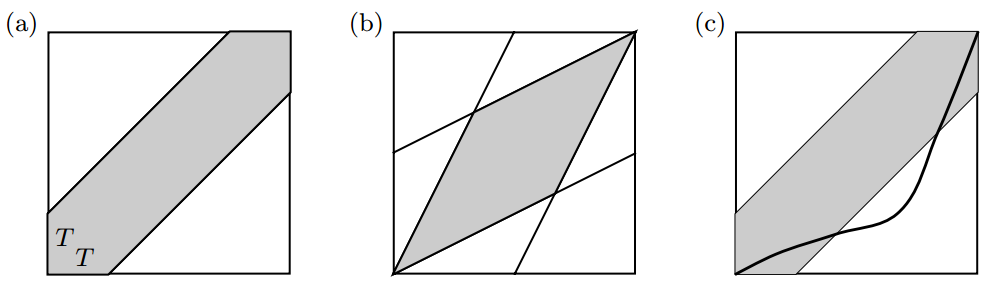
\includegraphics[width=15cm]{p7.png}
\caption{{\bf (a)} Полоса Сакоэ-Шиба ширины T; {\bf (b)} Параллелограмм Итакура при $S=2$; {\bf (c)} Искажающий путь, частично лежащий вне глобального ограничивающего региона.}
\label{fig:p7}
\end{figure}

Полоса Сакоэ-Шиба проходит вдоль главной диагонали и имеет фиксированную ширину $T$. Это означает, что элементы $x_i$ и $y_j$ могут быть поставлены в соответствие только если $j \in [{{m-T}\over{n-T}} \cdot i - T,{{m-T}\over{n-T} }\cdot i + T] \cap [1,\dots,m]$ (рис. \ref{fig:p7}a). Параллелограмм Итакура описывает регион, который ограничивает наклон искажающего пути. Более формально, для фиксированного $S \in {\rm I\!R}_{>1}$ параллелограмм Итакура состоит из всех ячеек, являющихся элементами каких-либо искажающих путей с наклоном от $1 \over S$ до $S$ (рис. \ref{fig:p7}b). Заметим также, что локальное ограничение на размер шага также вводит некоторый вид глобального ограничения. Например, рассматривавшееся выше ограничение $p_i-p{i-1} \in \{(2,1),(1,2),(1,1)\}$ для $i \in [2,\dots,l],$ является синонимом глобального ограничения в виде параллелограмма Итакуры с $S=2.$

Для глобального ограничивающего региона $R$, путь $p_R^*$ вычисляется практически таким же образом, как оптимальный искажающий путь в задаче без ограничений. Единственным отличием является то, что $c(x_i,y_j)$ полагается равным $\infty$ для всех пар $(i,j) \notin R$. Таким образом, требуется вычисление лишь тех ячеек матрицы кумулятивного расстояния, которые лежат в $R$. Это может значитально ускорить вычисление алгоритма DTW. Например, в случае полосы Сакоэ-Шиба фиксированной ширины $T$, потребуется лишь $O(T \cdot \max(n,m))$ времени вместо $O(nm)$ в классическом алгоритме DTW, что может привести к значительной экономии времени работы в случае $T \ll n,m.$

Однако, использование глобальных ограничений может быть нежелательным в некоторых случаях, поскольку оптимальный искажающий путь может выходить за рамки выбранного региона, и, таким образом, не совпадать с $p_R^*$ (см. \ref{fig:p7}c). В некоторых случаях это может привести к нежелательным или полностью бесполезным результатам.

\subsubsection{Алгоритм derivative dynamic time warping}
\subsection{Алгоритмы кластеризации}
\subsubsection{Примеры задач кластеризации}
\subsubsection{Эвристические графовые алгоритмы кластеризации}
\subsubsection{Статистические алгоритмы кластеризации}
\subsubsection{Алгоритмы иерархической кластеризации}
\subsubsection{Самоорганизующиеся карты Кохонена}
\section{Численные эксперименты}
\subsection{Поиск паттерна в истории котировок}
\subsection{Кластеризация фрагментов историй котировок}
\subsection{Построение полностью автоматизированной торговой стратегии}
\addcontentsline{toc}{section}{Введение}
\section*{Заключение}
\newpage{}
\bibliography{bibliography}
\end{document}